\chapter{Implementation}

Part of this thesis is to implement the asynchronous duet benchmark super-harness that takes an existing benchmark harness as an input and executes its benchmarks in the asynchronous duet style.
This kind of tool should greatly simplify the general use of the asynchronous duet method.

% Running in docker and reasons for it
To keep a configuration portable and the dependencies minimal we have decided to use the container technology, namely Docker~\cite{merkel2014docker} or Podman~\footnote{\url{https://podman.io/}, July 2022}.
Tool is named \lstinline{duetbench} and it is part of open sourced~\footnote{Apache Licence 2.0} python package \lstinline{duet}~\footnote{\url{https://github.com/TomasDrozdik/asynchronous-duet}, July 2022} that also implements other complementary tools described in~\cref{sec:result_parsing}.
Source code is available as an attachment to this thesis~\xxx{ref} and it has documentation in form of GitHub wiki~\cite{wiki}.

% Docker -> different environment -> support for both sequential and synchronous duet runs
Since one of the goals of this thesis is to compare asynchronous duet with synchronous and sequential method usage of containers makes direct comparison with~\citet{bulej2020duet} unreasonable.
Therefore \lstinline{duetbench} supports all three benchmarking methods in a containerized environment.

\section{Architecture}

\Cref{fig:duetbench_sequence} depicts architecture of \lstinline{duetbench} script.
\lstinline{duetbench} is a process on the host machine that spawns subprocesses that run containers --- one for each version A/B.
Since initialization of a container might take longer \lstinline{duetbench} waits for both containers to start and then uses \lstinline{docker exec}~\footnote{\lstinline{docker exec} reference \url{https://docs.docker.com/engine/reference/commandline/exec/}, July 2022} to run the command that executes the benchmark harness loop from~\cref{alg:harness}.
Then once both benchmarks finish, copy the raw result of those benchmarks from their respective containers and store them in some fixed format to preserve information about a particular run.
Afterward, stop and clean up both containers.
We refer to this process is as a \emph{run} and it is analogous to a \emph{trial} from~\citet{laaber2019software} and~\citet{abedi2017conducting}.
The distinction is that one \emph{run} can run 2 benchmarks in parallel in case of a duet run, but it may also run just a single benchmark in case of sequential run.

\begin{figure}
	\centering
	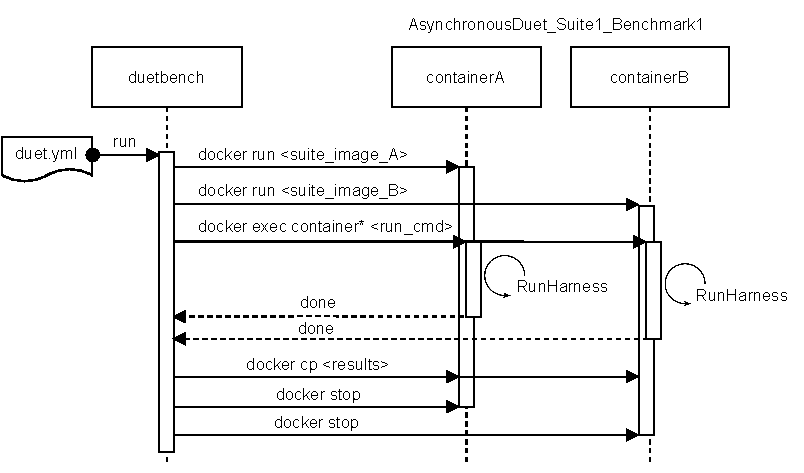
\includegraphics[width=\linewidth]{./figures/duetbench-sequence.drawio.pdf}
	\caption{
        UML sequence diagram of how \lstinline{duetbench} executes a single A/B asynchronous duet benchmark.
        All the parameters in angled brackets are specified in the configuration file \lstinline{duet.yml} described in~\cref{sec:configuration}.
        Note that the docker commands are simplified for brevity.
	}
	\label{fig:duetbench_sequence}
\end{figure}

If there are more benchmarks to execute pick the next one (according a particular scheduling strategy, see~\cref{sec:scheduling}) and do the same process.
In the case of the sequential method, the process is very much the same just omit the second container entirely and run them separately.

\subsection{Synchronized duet in containerized environment}

In the case of the synchronized duet, the benchmark harness needs to be modified as in~\citet{bulej2020duet}.
Additionally,~\citet{bulej2020duet} synchronize the iterations using shared memory barrier placed in \lstinline{/dev/shm} before benchmarks are started.
Then each benchmark invocation gets a path to this shared barrier file and their harness blocks on this barrier before each iteration.
To facilitate similar behavior between containers \lstinline{duetbench} starts the dockers with mounted volumes \lstinline{-v /dev/shm:/dev/shm} and shared inter process communication namespace \lstinline{--ipc host}~\footnote{\lstinline{docker run} reference \url{https://docs.docker.com/engine/reference/run/}, July 2022}.
Last but not least, something has to create this shared memory barrier and clean it up afterward.

Barrier is made with \lstinline{pthread_barrier_init}~\footnote{\lstinline{man 3 pthread_barrier_init}}, however this call is not available on all Unixes for example macOS~\footnote{macOS Monterey Version 12.3.1}.
Instead, \lstinline{duetbench} creates these barriers from one of the containers, since both have mounted the same volume \lstinline{/dev/shm}.
The advantage of such an approach is that docker containers access to \lstinline{pthread_barrier_init} even though the underlying host might not~\footnote{Since Docker on both macOS and Windows still runs Linux VM underneath docker containers \url{https://www.docker.com/blog/the-magic-behind-the-scenes-of-docker-desktop/}, July 2022}.

\subsection{Run Scheduling}
\label{sec:scheduling}

\lstinline{duetbench} supports two options for \emph{run scheduling}:
\begin{description}
    \item[Sequential] where benchmarks are run in order of definition from configuration file.
    \item[Randomized Interleaving Trials] where it randomly interleaves the runs from a configuration file.
        Hence it can mix different types of measurement methods and benchmarks.
        With multiple repetitions of a given measurement method it is essentially RMIT\cite{abedi2017conducting}.
\end{description}

\section{Configuration}
\label{sec:configuration}

\Cref{lst:config} shows section of \lstinline{duetbench} YAML configuration file that describes an A/B asynchronous duet and sequential run.
The goal of the design was to make configuration generic and simple to use so that many harnesses and benchmark suites can be adapted to use with \lstinline{duetbench}.
Full documentation of the \lstinline{duetbench} configuration including description of how to run synchronized duets not present in the~\cref{lst:config} is on the wiki~\cite{wiki}.

Freedom in run command allows for tweaking of the harness to better suite asynchronous duet, for example, some harnesses support skips of validation or various garbage collector options.
Detailed configuration of experiments is in~\cref{sec:benchmark_configuration}.

\begin{listing}
    \begin{lstlisting}
avrora:
  image: dacapo
  duet_repetitions: 2
  sequential_repetitions: 2
  schedule: randomized_interleaving_trials
  A:
    run: java -jar dacapo-A.jar -n 50 -o results.csv avrora
  B:
    run: java -jar dacapo-B.jar -n 50 -o results.csv avrora
  results:
    - results.csv
    \end{lstlisting}
    \caption{
        Example part of YAML configuration file for \lstinline{duetbench} that runs \lstinline{avrora} benchmark from the DaCapo suite.
        In this case, both A and B versions are packaged in a single container image as Java JAR archives.
        Run command specifies how to invoke the DaCapo harness --- 50 iterations, results in \lstinline{results.csv} and run only \lstinline{avrora} benchmark.
        All the result files or directories need to be specified in \lstinline{results} array field.
        Note the correspondence between user input fields from this configuration and parameters in angled brackets from~\cref{fig:duetbench_sequence}.
        Furthermore, users can specify the number of repetitions for both asynchronous duet and sequential measurements, as well as the scheduling strategy for those runs.
    }
    \label{lst:config}
\end{listing}

\section{Result parsing}
\label{sec:result_parsing}

Once a run finishes, results are copied in their raw format to a dedicated result directory on the host machine.
Results are then processed to some common format for further analysis.
For this purpose \lstinline{duet} package has \lstinline{duetprocess} script~\cite{wiki}.
It takes an output directory of \lstinline{duetbench} and produces single results file in CSV format.

The minimal schema of a result data point looks like this:
\begin{itemize}
    \item Directly parsed by \lstinline{duetprocess}:
        \begin{itemize}
            \item suite
            \item benchmark
            \item run: repetetion id, not necessarily run in order
            \item pair
            \item pair order: which pair was started first
            \item iteration
            \item \emph{artifacts}: \lstinline{duetbench} provides an option to run some additional commands such as \lstinline{lscpu} or \lstinline{cat /proc/meminfo} to obtain information about host environment
        \end{itemize}
    \item Specific per benchmark suite parsers:
        \begin{itemize}
            \item iteration start absolute timestamp (ns)
            \item iteration end absolute timestamp (ns)
        \end{itemize}
\end{itemize}

Since different benchmark suites have widely different results formats users have to write a parser plugin --- python function.
The parser has to obtain iteration start and end absolute timestamps from benchmark results. 
Additionally, since users need to write a parser for a given benchmark suite, they might add any sort of data that the benchmark produces as an addition to the above-mentioned schema.

Some benchmark suites don't track absolute timestamps of iterations and thus need some modification.
However, without absolute timestamps, one could not evaluate how iterations overlap (\emph{RQ2}).

\subsection{Notation}
\label{sec:notation}

To describe parsed results more formally and describe terminology from the \lstinline{duet} package we use following terms:

\begin{description}
    \item[Environment] $e \in E$ classifies host hardware and software configuration --- where \lstinline{duetbench} runs.
        Environment is deduced from artifacts in the above schema.
        Set of environments $E$ used in our experiments is described in~\cref{sec:experiment_setup}.
    \item[Type] $t \in T$ is the measurement method type where $T = \{seqn, sduet, aduet\}$ for sequential, synchronous duet and asynchronous duet respectively.
    \item[Pair] $p \in P$ is version of tested software in case of A/B runs $P = \{A, B\}$
    \item[Benchmark] $b \in B$ is a benchmark from a benchmark suite, formally $B = \{(suite, benchmark) | suite \in Suites, benchmark \in suite\}$
    \item[Run] in environment $e \in E$, of type $t \in T$, running benchmark $b \in B$ and pair $p \in P$ is denoted as $R^{e, t, b, p}$.
        It is a unit that \lstinline{duetbench} works with and can repeat multiple times.
    \item[Iteration] of a run $R^{e, t, b, p}$ with $iters$ iterations is an ordered set $(i_1, i_2, \dots i_{iters})$ of scores of particular benchmark --- execution time in nanoseconds.
        The duration of an iteration is a data point of an experiment.
\end{description}

To compare runs between environments we won't mix results from different environments and refer to an experiment $M^e$ in an environment $e \in E$ with some number of runs $runs$ per benchmark as set of runs:
\[M^e = \{R^{t, b, p}_r | t \in T, b \in B, p \in P \forall r \in \{1 \dots runs\}\}\]

To distinguish different measurement methods for some benchmark $b \in B$, denote a set of all sequential runs as
\[R^{seqn, b} = \{R^{t, b, p}_r | t = seqn, p \in P \forall r \in \{1 \dots runs\}\}\]
set of all synchronized duet measurements which are naturally paired on the level of pairs and iterations as
\begin{align*}
R^{sduet, b} &= \{(R^{t, b, A}_r, R^{t, b, B}_r) | t = sduet, p \in P \forall r \in \{1 \dots runs\}\} \\
             &= \{((i^A_j, i^B_j)_r) | \forall r \in \{1 \dots runs\}, \forall j \in \{1 \dots iters\}\}
\end{align*}
and finaly set of all asynchronous duet measurements, naturally paired on the level of pairs as
\[R^{aduet, b} = \{(R^{t, b, A}_r, R^{t, b, B}_r) | t = aduet \forall r \in \{1 \dots runs\}\}\]

\subsection{Overlaps}
\label{sec:overlaps}

To address \emph{RQ2} \lstinline{duetprocess} provides a method to compute overlaps of iterations of given asynchronous duet run.
Let $(R_A, R_B) \in R^{aduet, b}$ represent asynchronous duet A/B runs of some benchmark $b \in B$.
Iterations of respective run are $R_A = (i^A_1 \dots i^B_{iters})$ and $R_B = (i^A_1 \dots i^B_{iters})$.
Then an overlap of these two runs $O_{R_A, R_B}$ can be expressed as:
\begin{align*}
start(i) &= \text{start of iteration }i \\
end(i) &= \text{end of iteration } i \\
overlap\_start(i_1, i_2) &= max(start(i_1), start(i_2)) \\
overlap\_end(i_1, i_2) &= min(end(i_1), end(i_2)) \\
O_{R_A, R_B} =& \{(i^A_i, i^B_j) | overlap\_start(i^A_i, i^B_j) < overlap\_end(i^A_i, i^B_j) \\
              &\forall i \in \{1 \dots iters\}, \forall j \in \{1 \dots iters\}\} \\
\end{align*} 

However, not all overlaps are equaly important.
As shown in~\cref{fig:overlap_timeline} and \emph{RQ2} introduction some overlaps might be really small and cover start of one iteration with the end of another.
Following notations are used to express quality of an overlap:

\xxx{TODO: add weighted overlaps versions}
\begin{align*}
overlap\_time(i_1, i_2) &= overlap\_end(i^1_i, i^2_j) - overlap\_start(i^1_i, i^2_j) \\
\end{align*}

A set of all overlaps $O^{M^e}$ of an experiment $M^e$ is
\[O^{M^e} = \{(O_{R_A, R_B}) | (R_A, R_B) \in R^{aduet, b} \forall b \in B \}\]
